\chapter{SYSTEM ARCHITECTURE AND METHODOLOGY}

\section{System Overview}

The proposed system estimates the location of a mountain image by comparing its skyline with a database of reference skylines generated from a \gls{dem}. Before localization, the system prepares the reference skyline database and trains the skyline segmentation model using a synthetic dataset. During localization, the input image is processed to extract its skyline, which is then matched against the reference database to estimate the camera location.

The system consists of five main modules. The first module generates the reference skyline database from the terrain model. The second module generates a synthetic dataset used to train the segmentation model. The third module separates the sky from the terrain in the query image. The fourth module converts the segmented mask into a skyline profile. The final module compares the extracted skyline with the reference database and returns the best matching location.

Figure~\ref{fig:system_pipeline} shows the complete workflow of the proposed system.

\begin{figure}[H]
\centering
\begin{adjustbox}{max totalsize={0.95\textwidth}{0.72\textheight},center}
\begin{tikzpicture}[
>=Latex,
node distance=13mm,
font=\small,
block/.style={
draw,
rounded corners=2pt,
minimum width=42mm,
minimum height=9mm,
align=center
},
line/.style={->,thick}
]

\node[block] (dem) {Copernicus GLO-30\\\gls{dem}};

\node[block,below=of dem] (db)
{Reference Skyline\\Database Generation};

\node[block,right=54mm of db] (dataset)
{Synthetic Query\\Dataset Generation};

\node[block,below=of dataset]
(train)
{Train Skyline\\Segmentation Model};

\node[block,below=24mm of db]
(query)
{Query Image};

\node[block,below=of query]
(segment)
{Skyline\\Segmentation};

\node[block,below=of segment]
(extract)
{Skyline\\Extraction};

\node[block,below=of extract]
(match)
{Skyline\\Matching};

\node[block,below=of match]
(location)
{Estimated\\Location};

\draw[line] (dem)--(db);
\draw[line] (dem)-| (dataset);
\draw[line] (dataset)--(train);
\draw[line] (query)--(segment);
\draw[line] (segment)--(extract);
\draw[line] (extract)--(match);
\draw[line] (match)--(location);

% Route cross-branch links outside nodes with clear source/target anchors.
\coordinate (to_match) at ($(match.east)+(12mm,0)$);
\draw[line] (db.east) -| (to_match) -- (match.east);

\coordinate (to_segment) at ($(segment.east)+(12mm,0)$);
\draw[line] (train.south) |- (to_segment) -- (segment.east);

\end{tikzpicture}
\end{adjustbox}
\caption{Overall workflow of the proposed skyline-based localization system.}
\label{fig:system_pipeline}
\end{figure}

The preparation modules are executed once for the selected study area. The generated skyline database and trained segmentation model are then reused for every localization query. During localization, only the query image is required as input. The estimated location is obtained by matching the extracted skyline against the reference skyline database.

\section{Study Area}

The proposed system is developed for the Khumbu region of eastern Nepal. This region contains steep terrain, deep valleys, and distinctive mountain skylines that are well suited for skyline-based localization. The study area also includes several popular trekking routes where \gls{gnss} signals may be unreliable because of terrain obstruction.

Terrain information is obtained from the Copernicus GLO-30 \gls{dem}. The dataset provides an approximate spatial resolution of 30~m and is used throughout the project. The same terrain model is used to generate the reference skyline database and the synthetic training dataset. Using a single terrain source keeps every stage of the system consistent.

The study area is defined before database generation. Only viewpoints located inside the selected boundary are used when generating reference skylines. Restricting the search area reduces the database size while ensuring that every reference skyline corresponds to a valid location within the study region.

Figure~\ref{fig:study_area} shows the selected study area.

\begin{figure}[H]
    \centering
    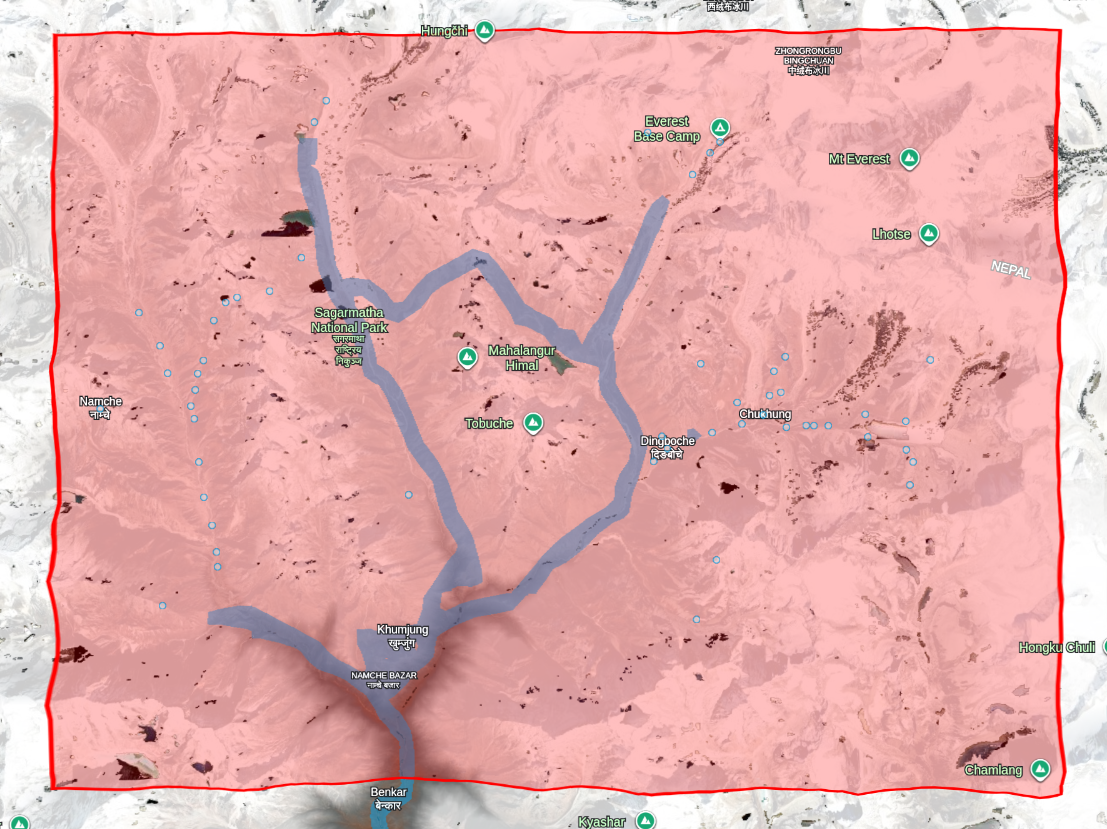
\includegraphics[width=0.8\textwidth]{src/images/roi.png}
    \caption{Study area used for reference skyline generation and system evaluation.}
    \label{fig:study_area}
\end{figure}

\section{Reference Skyline Database}

The reference skyline database contains the skyline profile associated with every valid viewpoint in the study area. During localization, the extracted skyline from the query image is compared against this database to estimate the camera location. Since the database is generated only once, the computational cost of skyline generation does not affect localization time.

The database generation process begins by selecting viewpoints across the study area. A skyline profile is generated for every viewpoint using the terrain model. Viewpoints that do not contain sufficient terrain variation are removed before the remaining profiles are stored in the database.

Figure~\ref{fig:database_generation} illustrates the complete database generation process.

\begin{figure}[H]
\centering
\begin{adjustbox}{max totalsize={0.95\textwidth}{0.72\textheight},center}
\begin{tikzpicture}[
>=Latex,
node distance=11mm,
font=\small,
block/.style={
draw,
rounded corners=2pt,
minimum width=42mm,
minimum height=9mm,
align=center
},
line/.style={->,thick}
]

\node[block] (dem){Copernicus GLO-30\\\gls{dem}};

\node[block,below=of dem](viewpoints){Generate\\Viewpoints};

\node[block,below=of viewpoints](skyline){Generate\\Skyline Profiles};

\node[block,below=of skyline](filter){Filter Invalid\\Profiles};

\node[block,below=of filter](database){Reference Skyline\\Database};

\draw[line](dem)--(viewpoints);
\draw[line](viewpoints)--(skyline);
\draw[line](skyline)--(filter);
\draw[line](filter)--(database);

\end{tikzpicture}
\end{adjustbox}
\caption{Reference skyline database generation process.}
\label{fig:database_generation}
\end{figure}

\subsection{Viewpoint Generation}

The study area is sampled using a regular grid. Each grid point represents a candidate camera location from which a skyline profile is generated. The spacing between neighbouring viewpoints is fixed during database generation so that the study area is sampled uniformly.

The elevation of every viewpoint is obtained directly from the \gls{dem}. The viewpoint coordinates are also recorded because they are required after skyline matching to recover the estimated camera location.

\subsection{Skyline Generation}

A skyline profile is generated for every viewpoint using the surrounding terrain. The skyline represents the highest visible terrain elevation in every viewing direction.

The horizon is sampled over the complete $360^\circ$ field of view. For every azimuth direction, the terrain elevation angle is computed from the observer to the visible terrain. The highest elevation angle becomes the skyline value for that direction.

The elevation angle is computed as

\begin{equation}
\theta=\tan^{-1}\left(\frac{h_t-h_o}{d}\right),
\label{eq:elevation_angle}
\end{equation}

where $h_t$ is the terrain elevation, $h_o$ is the observer elevation, and $d$ is the horizontal distance between the observer and the terrain point.

Repeating this process for all azimuth directions produces a one-dimensional skyline profile that describes the visible terrain surrounding the viewpoint.

Algorithm~\ref{alg:skyline_generation} summarizes the skyline generation procedure.

\begin{algorithm}[!ht]
\caption{Reference Skyline Generation}
\label{alg:skyline_generation}
\begin{algorithmic}[1]
\Require Observer location, terrain model
\Ensure Skyline profile
\ForAll{azimuth directions}
\State Trace the terrain profile
\State Compute the elevation angle of visible terrain points
\State Select the maximum elevation angle
\State Append the value to the skyline profile
\EndFor
\State \Return the skyline profile
\end{algorithmic}
\end{algorithm}

\subsection{Skyline Filtering}

Not every generated skyline is suitable for localization. Viewpoints located on flat terrain often produce skyline profiles with little variation. These profiles appear similar at many different locations and reduce matching accuracy.

Each skyline profile is evaluated before being added to the database. Profiles with insufficient variation are removed using a minimum elevation-angle condition so that very flat and uninformative profiles are excluded.

Removing unsuitable viewpoints reduces the database size while improving the distinctiveness of the remaining skyline profiles.

\subsection{Database Storage}

The remaining skyline profiles are stored together with the corresponding viewpoint information. Each database entry contains the viewpoint coordinates and the associated skyline profile.

The database is loaded during localization and searched using the extracted skyline profile from the query image. Since every stored profile corresponds to a known viewpoint, the location of the best matching profile becomes the estimated camera location.

\section{Synthetic Query Dataset}

A labelled dataset is required to train the skyline segmentation model. Since no suitable labelled mountain image dataset is available for the study area, the training data is generated automatically. The synthetic dataset provides paired RGB images and ground truth sky masks without manual annotation.

The dataset is generated from the same terrain model used for the reference skyline database. This ensures that the terrain observed during training is consistent with the terrain used during localization. Every generated image has a corresponding binary sky mask and ground truth viewpoint information.

Figure~\ref{fig:synthetic_dataset_pipeline} shows the dataset generation process.

\begin{figure}[H]
\centering
\begin{adjustbox}{max totalsize={0.95\textwidth}{0.72\textheight},center}
\begin{tikzpicture}[
>=Latex,
node distance=11mm,
font=\small,
block/.style={
draw,
rounded corners=2pt,
minimum width=42mm,
minimum height=9mm,
align=center
},
line/.style={->,thick}
]

\node[block] (dem){Copernicus GLO-30\\\gls{dem}};

\node[block,right=40mm of dem](texture){Satellite\\Texture};

\node[block,below=18mm of dem](render){Synthetic Scene\\Rendering};

\node[block,below=of render](image){RGB\\Image};

\node[block,right=40mm of image](mask){Binary\\Sky Mask};

\node[block,below=18mm of image](dataset){Synthetic\\Dataset};

\draw[line](dem)--(render);
\draw[line](texture)--(render);
\draw[line](render)--(image);
\draw[line](render)--(mask);
\draw[line](image)--(dataset);
\draw[line](mask)--(dataset);

\end{tikzpicture}
\end{adjustbox}
\caption{Synthetic dataset generation process.}
\label{fig:synthetic_dataset_pipeline}
\end{figure}

\subsection{Scene Generation}

Synthetic mountain scenes are rendered using the terrain model and satellite imagery. The terrain geometry is obtained from the Copernicus GLO-30 \gls{dem}, while the satellite image is mapped onto the terrain surface as a texture.

The virtual camera is positioned at viewpoints distributed throughout the study area. For each viewpoint, the terrain is rendered from the camera perspective to produce a synthetic RGB image. Since the viewpoint is known during rendering, the corresponding camera location is also recorded.

This process is repeated until the required number of training samples has been generated.

\subsection{Automatic Sky Mask Generation}

The sky mask is generated directly from the rendered scene. Since the terrain model is completely known, the system can identify whether each pixel belongs to the sky or the terrain.

The generated mask is stored as a binary image. Sky pixels are assigned a value of 0, while terrain pixels are assigned a value of 255. Every RGB image has one corresponding binary mask, producing perfectly aligned training pairs without manual annotation.

The generated masks are later used as the ground truth labels during segmentation model training.

\subsection{Ground Truth Storage}

Each generated sample is accompanied by its corresponding viewpoint information. The dataset stores the RGB image, binary mask, and camera information using the same sample identifier.

The generated images and masks are stored separately, while the viewpoint information is recorded in a ground truth file. This organization allows the images, masks, and viewpoint information to be loaded independently during model training and system evaluation.

\section{Skyline Segmentation}

The first step of localization is separating the sky from the surrounding terrain. The resulting binary mask is used to extract the skyline profile for matching. Since mountain images often contain snow, shadows, clouds, and changing illumination, simple image processing techniques do not produce reliable results. A deep learning model is used to perform the segmentation.

To improve generalization beyond purely synthetic scenes, the segmentation stage is also informed by examples from the GeoPose3K benchmark \cite{brejcha2019geopose3k}. GeoPose3K provides real mountain photographs with known camera poses, making it useful for exposing the model to realistic skyline boundaries, lighting variation, and terrain appearance that are difficult to capture through rendering alone.

The segmentation process consists of three stages. First, the input image is processed by a U-Net model to predict the sky region. Next, the predicted mask is converted into a binary image. Finally, connected component analysis and edge refinement are applied to improve the skyline boundary.

Figure~\ref{fig:segmentation_pipeline} illustrates the segmentation process.

\begin{figure}[H]
\centering
\begin{adjustbox}{max totalsize={0.95\textwidth}{0.72\textheight},center}
\begin{tikzpicture}[
>=Latex,
node distance=11mm,
font=\small,
block/.style={
draw,
rounded corners=2pt,
minimum width=36mm,
minimum height=9mm,
align=center
},
line/.style={->,thick}
]

\node[block](image){Input\\Image};

\node[block,below=of image](unet){U-Net\\Prediction};

\node[block,below=of unet](component){Connected\\Components};

\node[block,below=of component](edge){Canny Edge\\Refinement};

\node[block,below=of edge](mask){Final\\Sky Mask};

\draw[line](image)--(unet);
\draw[line](unet)--(component);
\draw[line](component)--(edge);
\draw[line](edge)--(mask);

\end{tikzpicture}
\end{adjustbox}
\caption{Skyline segmentation process.}
\label{fig:segmentation_pipeline}
\end{figure}

\subsection{Sky Segmentation}

The input image is resized before being passed to the segmentation model. The model predicts the probability that each pixel belongs to the sky. The predicted probability map is converted into a binary mask using a fixed threshold.

This produces an initial estimate of the sky region. Although the overall sky boundary is usually detected correctly, small segmentation errors may still appear around mountain ridges.

\subsection{Mask Refinement}

The predicted mask is refined before skyline extraction. The first refinement step removes disconnected sky regions using connected component analysis. Only sky regions connected to the top boundary of the image are retained.

The skyline boundary is then refined using Canny edge detection. For every image column, the detected skyline is adjusted to the nearest edge within a local search window. This improves the alignment between the predicted skyline and the visible mountain ridge.

The final output is a binary image where sky pixels have a value of 0 and terrain pixels have a value of 255. This mask is passed to the skyline extraction stage.

\section{Skyline Extraction}

The segmented sky mask is converted into a one-dimensional skyline profile before localization. Instead of comparing binary images directly, the system represents the skyline as a sequence of elevation angles. This representation is independent of image resolution and can be compared directly with the reference skyline database.

The skyline extraction process consists of three steps. First, the skyline boundary is detected from the binary mask. Next, the detected boundary is converted into elevation angles using the camera model. Finally, the resulting profile is validated before matching.

Figure~\ref{fig:skyline_extraction_pipeline} shows the skyline extraction process.

\begin{figure}[H]
\centering
\begin{adjustbox}{max totalsize={0.95\textwidth}{0.72\textheight},center}
\begin{tikzpicture}[
>=Latex,
node distance=11mm,
font=\small,
block/.style={
draw,
rounded corners=2pt,
minimum width=38mm,
minimum height=9mm,
align=center
},
line/.style={->,thick}
]

\node[block](mask){Binary\\Sky Mask};

\node[block,below=of mask](detect){Detect\\Skyline};

\node[block,below=of detect](convert){Convert to\\Elevation Angles};

\node[block,below=of convert](validate){Validate\\Profile};

\node[block,below=of validate](profile){Skyline\\Profile};

\draw[line](mask)--(detect);
\draw[line](detect)--(convert);
\draw[line](convert)--(validate);
\draw[line](validate)--(profile);

\end{tikzpicture}
\end{adjustbox}
\caption{Skyline extraction process.}
\label{fig:skyline_extraction_pipeline}
\end{figure}

\subsection{Skyline Detection}

The skyline is extracted independently for every image column. Starting from the top of the binary mask, the first terrain pixel is identified and recorded as the skyline position. If no terrain pixel is found in a column, the bottom of the image is used.

Small discontinuities caused by segmentation errors are removed using a median filter. This smooths the extracted skyline while preserving the overall terrain shape.

\subsection{Elevation Angle Computation}

The detected skyline is represented as image coordinates. These coordinates are converted into viewing rays using the camera field of view and image dimensions.

The elevation angle of each viewing ray is computed as

\begin{equation}
\theta=\sin^{-1}(r_y),
\end{equation}

where $r_y$ is the vertical component of the normalized viewing ray.

The corresponding azimuth angle is computed as

\begin{equation}
\phi=\tan^{-1}\left(\frac{r_x}{-r_z}\right),
\end{equation}

where $r_x$ and $r_z$ are the horizontal components of the viewing ray.

The skyline profile is interpolated onto a uniform azimuth grid before matching. Uniform sampling ensures that every query profile can be compared directly with the reference skyline database.

\subsection{Profile Validation}

Some images contain very little visible terrain. These images produce skyline profiles with almost no variation and are unsuitable for localization.

Before matching, every extracted profile is checked for sufficient terrain variation. Profiles that do not satisfy the required variation are discarded. This prevents unreliable skyline profiles from producing incorrect localization results.

\section{Skyline Matching}

The extracted skyline profile is compared with the reference skyline database to estimate the camera location. Since the database contains a large number of skyline profiles, the matching process is divided into two stages. The first stage removes unlikely candidates using fast correlation, while the second stage performs detailed alignment on the remaining candidates.

Figure~\ref{fig:matching_pipeline} illustrates the skyline matching process.

\begin{figure}[H]
\centering
\begin{adjustbox}{max totalsize={0.95\textwidth}{0.72\textheight},center}
\begin{tikzpicture}[
>=Latex,
node distance=11mm,
font=\small,
block/.style={
draw,
rounded corners=2pt,
minimum width=40mm,
minimum height=9mm,
align=center
},
line/.style={->,thick}
]

\node[block](query){Query\\Skyline};

\node[block,below=of query](fft){FFT-based\\Correlation};

\node[block,below=of fft](candidate){Top\\Candidates};

\node[block,below=of candidate](dtw){FastDTW\\Refinement};

\node[block,below=of dtw](ranking){Candidate\\Ranking};

\node[block,below=of ranking](location){Estimated\\Location};

\draw[line](query)--(fft);
\draw[line](fft)--(candidate);
\draw[line](candidate)--(dtw);
\draw[line](dtw)--(ranking);
\draw[line](ranking)--(location);

\end{tikzpicture}
\end{adjustbox}
\caption{Skyline matching process.}
\label{fig:matching_pipeline}
\end{figure}

\subsection{Feature Extraction}

The skyline profile alone does not fully describe the terrain shape. To capture both the overall skyline and local changes, three feature sequences are computed from every profile. These consist of the normalized skyline profile together with its first and second derivatives.

Each feature is normalized before matching. This reduces the effect of differences in elevation magnitude while preserving the overall skyline shape.

\subsection{Candidate Selection}

The first stage compares the query skyline with every reference skyline using cross-correlation. The correlation scores obtained from the three feature sequences are combined into a single similarity score.

Because a query photo covers only a limited field of view while each reference skyline covers 360\textdegree, the query profile is evaluated at multiple azimuth offsets over the full reference profile. This sliding-window correlation step finds the best matching azimuth window before detailed refinement.

The best correlation also provides the rotational alignment between the query skyline and the reference skyline. If compass information is available, only rotations close to the measured heading are considered. This reduces the search space and removes unlikely candidates.

To reduce computation, an initial search is performed using a subset of viewpoints. Only the strongest candidates are selected for detailed matching.

\subsection{Profile Alignment}

The selected candidates are refined using \gls{dtw}. Unlike direct point-by-point comparison, \gls{dtw} allows small local differences between skyline profiles while preserving the overall terrain shape.

The alignment cost produced by \gls{dtw} measures the similarity between the query skyline and each candidate skyline. Lower alignment costs indicate better matches.

\subsection{Candidate Ranking}

Each candidate contains a correlation score and a \gls{dtw} alignment cost. These two measures are combined to rank the candidate locations.

The candidate with the highest overall similarity is selected as the final localization result. The coordinates associated with the selected reference skyline are returned as the estimated camera location.

% \chapter{SYSTEM ARCHITECTURE AND METHODOLOGY}
% \label{chap:methodology}

% \section{Design Considerations}

% The proposed system is designed for visual geolocation in mountainous terrain. The design is based on the characteristics of the Khumbu region and the goal of estimating a user's location from a single mountain photograph. This section explains the main design decisions used in the system.

% \begin{enumerate}
%     \item \textbf{Localization in Mountain Valleys}

%     The system is designed for mountain valleys instead of open mountain peaks. In many valleys, the surrounding mountains block \gls{gnss} signals and reduce positioning accuracy. These mountains also produce clear skyline shapes that can be used for visual localization. This makes valleys a suitable environment for the proposed system.

%     \item \textbf{Reference Database from a \gls{dem}}

%     Collecting reference photographs for every possible viewpoint is difficult and time-consuming. Instead, the system generates reference skylines directly from a \gls{dem}. Since the terrain does not change, the database only needs to be generated once for the selected study area. The same method can also be used in other mountain regions by using a different \gls{dem}.

%     \item \textbf{Fixed Search Distance}

%     The skyline does not continue to change as more distant terrain is included. Terrain that is very far from the observer usually contributes little useful information because it is hidden by nearer mountains or becomes difficult to see. For this reason, the maximum search distance is determined before generating the database. All reference skylines are then generated using this distance.

%     \item \textbf{Dense Viewpoint Sampling}

%     The system generates reference skylines from viewpoints spaced 30~m apart. A small spacing increases the chance that one of the reference skylines closely matches the query image. Viewpoints that provide little useful skyline information are removed before the database is stored. This reduces the database size without affecting localization.

%     \item \textbf{Synthetic Training Images}

%     A large labelled dataset of mountain skyline images is not available for the study area. To solve this problem, the system generates synthetic mountain images from the same \gls{dem} used to build the database. Since the terrain is already known, the sky masks are generated automatically. These image-mask pairs are used to train the skyline segmentation model.

%     \item \textbf{Two-Stage Skyline Matching}

%     Comparing a query skyline with every reference skyline using a detailed matching algorithm would take a long time. The system first performs a fast search to find the most likely candidates. A second matching stage then compares only these candidates in more detail. This reduces the computation time while maintaining localization accuracy.
% \end{enumerate}

% \section{Study Area}

% This study focuses on the Khumbu region of northeastern Nepal. The region includes Mount Everest and many other high mountain peaks. It also contains deep valleys where satellite-based positioning is often difficult. These valleys produce clear skyline shapes, making the region suitable for skyline-based localization.

% The study area covers approximately $40~\mathrm{km} \times 30~\mathrm{km}$, bounded by $86.582^\circ$E to $86.989^\circ$E longitude and $27.770^\circ$N to $28.041^\circ$N latitude. Figure~\ref{fig:roi} shows the selected study area.

% \begin{figure}[!ht]
%     \centering
%     
\includegraphics[width=0.75\linewidth]{figures/roi.png}
%     \caption{Region of Interest}
%     \label{fig:roi}
% \end{figure}

% Two Copernicus \glspl{dem} are used in this work. The Copernicus GLO-90 \gls{dem} is used to study the terrain and determine the maximum distance used for skyline generation. After the search distance is selected, the Copernicus GLO-30 \gls{dem} is used for the rest of the system. It is used to generate the reference skyline database, create the synthetic training dataset, and render the terrain during localization.

% \section{System Overview}

% The proposed system estimates the location of a mountain photograph using its skyline. Before localization can begin, the system prepares a reference database and trains a skyline segmentation model. These steps are performed once for the selected study area.

% The process begins by analyzing the study area using the Copernicus GLO-90 \gls{dem}. This analysis is used to determine the maximum search distance for skyline generation. The Copernicus GLO-30 \gls{dem} is then downloaded and used to generate the reference skyline database. The same terrain model is also used to create synthetic mountain images and sky masks for training the segmentation model.

% When a user provides a mountain photograph, the segmentation model first separates the sky from the terrain. The skyline is extracted from the predicted sky mask and converted into a one-dimensional skyline profile. This profile is then compared with the reference skyline database using a two-stage matching algorithm. The best matching skyline gives the estimated camera location.

% Figure~\ref{fig:system-overview} shows the complete workflow of the proposed system.

% \begin{figure}[htbp]
% \centering
% \begin{tikzpicture}[
%     node distance=1.2cm and 1.5cm,
%     font=\sffamily\small,
%     box/.style={
%         draw,
%         rectangle,
%         rounded corners=3pt,
%         minimum width=3.8cm,
%         minimum height=0.8cm,
%         align=center,
%         text width=3.6cm,
%         fill=gray!3,
%         draw=gray!60,
%         thick
%     },
%     database/.style={
%         draw,
%         cylinder,
%         shape border rotate=90,
%         minimum width=2.2cm,
%         minimum height=0.8cm,
%         align=center,
%         text width=2.0cm,
%         fill=blue!5,
%         draw=blue!50,
%         thick
%     },
%     line/.style={
%         draw,
%         -{Stealth[scale=1.0]},
%         thick,
%         gray!80!black
%     }
% ]

% \node[database] (dem) {Copernicus DEM\\(GLO-30)};

% \node[box, below left=1.0cm and 0.5cm of dem] (refgen) {Reference Skyline\\Generation};
% \node[box, below right=1.0cm and 0.5cm of dem] (syngen) {Synthetic Dataset\\Generation};

% \node[database, below=1.2cm of refgen] (refdb) {Reference Skyline\\Database};
% \node[box, below=1.2cm of syngen] (training) {U-Net\\Training};

% \node[box, left=2.2cm of refdb] (photo) {User Photograph};
% \node[box, below=1.2cm of photo] (extract) {Skyline\\Extraction};
% \node[box, below=3.2cm of refdb] (matching) {Hierarchical Matching\\(FFT + DTW)};
% \node[box, below=1.0cm of matching] (location) {Estimated\\User Location};

% \path[line] (dem) -| (refgen);
% \path[line] (dem) -| (syngen);

% \path[line] (refgen) -- (refdb);
% \path[line] (syngen) -- (training);

% \path[line] (photo) -- (extract);
% \path[line] (extract) |- (matching);

% \path[line] (refdb) -- (matching);
% \path[line] (training) |- (extract.east);

% \path[line] (matching) -- (location);

% \end{tikzpicture}
% \caption{Overall workflow of the proposed skyline-based visual geolocation system.}
% \label{fig:system_workflow}
% \end{figure}

% \section{Reference Skyline Database}

% The reference skyline database contains skyline profiles generated from known locations within the study area. During localization, the skyline extracted from the query image is compared with the profiles stored in this database. The location of the best matching profile is returned as the estimated camera position.

% The database is generated from the Copernicus GLO-30 \gls{dem}. Since the terrain does not change, the database only needs to be generated once. The same database is then reused for all localization queries.

% \subsection{Overview}

% The database generation process consists of four main steps. First, reference viewpoints are generated across the study area. Next, a skyline profile is generated for each viewpoint using ray casting. Skyline profiles that contain little terrain information are removed. Finally, the remaining profiles are stored together with the viewpoint information in a Parquet database.

% Algorithm~\ref{alg:skyline_database_generation} summarizes the complete database generation process.

% \begin{algorithm}[!ht]
% \caption{Reference Skyline Database Generation}
% \label{alg:skyline_database_generation}

% \KwIn{Copernicus GLO-30 \gls{dem}, study area}
% \KwOut{Reference skyline database}

% Generate reference viewpoints with 30~m spacing\;

% \ForEach{viewpoint}{
% Obtain the terrain elevation\;
% Place the observer 1.6~m above the terrain\;
% Generate a skyline profile using ray casting\;
% Filter the skyline profile\;
% Store the valid profile in the database\;
% }

% Save the database in Parquet format\;

% \end{algorithm}

% \subsection{Viewpoint Generation}

% Reference viewpoints are generated on a regular grid covering the study area. A spacing of 30~m is used between neighboring viewpoints. This provides dense coverage while keeping the database size manageable.

% The elevation of each viewpoint is obtained from the Copernicus GLO-30 \gls{dem}. An observer height of 1.6~m is added to the terrain elevation to represent the camera position during skyline generation.

% The complete study area contains a large number of viewpoints. Instead of processing all viewpoints at once, they are processed in batches of 4096. This reduces memory usage during database generation.

% \subsection{Skyline Generation}

% A skyline profile is generated for every reference viewpoint using the HORAYZON ray-casting library. Rays are cast in all directions around the observer with an angular interval of $1^\circ$. This produces a skyline profile containing 360 samples.

% For each viewing direction, the terrain is sampled until the maximum search distance of 30~km is reached. The highest visible terrain point along the ray defines the skyline for that direction.

% The elevation angle of each terrain sample is computed as

% \begin{equation}
% \theta=\tan^{-1}\left(\frac{h_t-h_o}{d}\right),
% \label{eq:elevation_angle}
% \end{equation}

% where $h_t$ is the terrain elevation, $h_o$ is the observer elevation, and $d$ is the horizontal distance from the observer.

% The skyline value for each viewing direction is the maximum elevation angle along the ray,

% \begin{equation}
% \theta_{\mathrm{sky}}=\max_i(\theta_i),
% \label{eq:skyline_max}
% \end{equation}

% where $\theta_i$ is the elevation angle of the $i^{\mathrm{th}}$ terrain sample.

% Repeating this process for all viewing directions produces the skyline profile

% \begin{equation}
% S=\left[\theta_0,\theta_1,\ldots,\theta_{359}\right].
% \label{eq:skyline_profile}
% \end{equation}

% Since every skyline profile uses the same angular interval and search distance, all profiles have the same length and can be compared directly during localization.

% Figure~\ref{fig:skyline_generation} illustrates the skyline generation process.

% \subsection{Skyline Filtering}

% Not every generated skyline is useful for localization. Some viewpoints produce almost flat skyline profiles with very little variation. These profiles are difficult to distinguish from one another and increase the database size without improving localization.

% Each skyline profile is evaluated before it is stored. The profile must satisfy two conditions. The standard deviation of the elevation angles must be at least $1.5^\circ$, and the maximum elevation angle must be at least $1.0^\circ$.

% \begin{equation}
% \sigma_S \ge 1.5^\circ,
% \end{equation}

% \begin{equation}
% \max(S)\ge1.0^\circ.
% \end{equation}

% Profiles that do not satisfy both conditions are discarded. This removes viewpoints with little terrain variation while keeping skyline profiles that are more useful for matching.

% \subsection{Database Storage}

% The remaining skyline profiles are stored in a Parquet database. Each record represents one reference viewpoint together with its corresponding skyline profile.

% The database stores the viewpoint longitude, latitude, ground elevation, skyline elevation angles, and their corresponding azimuth angles. Writing the database in batches avoids storing all viewpoints in memory during generation.

% Once the database has been generated, it is reused for every localization query. This allows the online localization stage to perform only skyline matching without generating new reference skylines.

% % Let $s$ be the horizontal distance from the viewpoint, $z(s)$ the terrain elevation, and $z_{\mathrm{cam}}$ the camera elevation. The elevation angle at distance $s$ is

% % \begin{equation}
% % \theta(s)=
% % \arctan
% % \left(
% % \frac{z(s)-z_{\mathrm{cam}}}{s}
% % \right).
% % \end{equation}

% % The skyline elevation angle for that direction is

% % \begin{equation}
% % \theta_h=
% % \max_{s\in(0,R_{\max}]}
% % \theta(s),
% % \end{equation}

% % where $R_{\max}=30\,\mathrm{km}$.

% % A visibility range of $30\,\mathrm{km}$ was selected because it captures the major mountain shapes required for localization while avoiding unnecessary computation at longer distances. Repeating this process for all 360 directions produces a complete skyline profile for the viewpoint.

% % Each skyline profile is stored together with the viewpoint coordinates and elevation to form the reference skyline database.

% % \begin{figure}[htbp]
% % \centering
% % \begin{tikzpicture}[font=\sffamily\small, scale=0.95]

% % % Draw Coordinate Grid
% % \draw[help lines, gray!20, step=1.0] (-1,-1) grid (10,5);

% % % Draw Axes
% % \draw[->, thick] (-0.5,0) -- (10.5,0) node[right] {Horizontal Distance $s$};
% % \draw[->, thick] (0,-0.5) -- (0,5.5) node[above] {Elevation $z$};

% % % Draw Terrain
% % \draw[very thick, brown!70!black, fill=brown!10] 
% %     (0,1.2) .. controls (1.5,1.5) and (2.5,0.8) .. (3.5,1.5)
% %     .. controls (4.5,2.2) and (5.5,3.2) .. (6.5,2.8)
% %     .. controls (7.5,2.4) and (8.5,4.5) .. (9.5,4.0)
% %     -- (10,0) -- (0,0) -- cycle;

% % % Viewpoint Observer
% % \coordinate (ObsBase) at (1.0, 1.35);
% % \coordinate (ObsCam) at (1.0, 2.5); % Camera height added
% % \draw[thick, blue] (ObsBase) -- (ObsCam);
% % \draw[fill=blue] (ObsCam) circle (0.08) node[left=2pt] {Observer $\mathbf{v}_i$};
% % \node[right, blue, font=\scriptsize] at (1.0, 1.9) {$h_{\text{cam}}$};

% % % Rays
% % \coordinate (T1) at (3.5, 1.5);
% % \coordinate (T2) at (6.0, 2.2);
% % \coordinate (T3) at (8.5, 3.8);

% % \draw[dashed, red!60, thin] (ObsCam) -- (T1);
% % \draw[dashed, red!60, thin] (ObsCam) -- (T2);
% % \draw[draw=green!60!black, thick, -{Stealth[scale=1.2]}] (ObsCam) -- (T3) node[midway, above left, black, font=\scriptsize] {Horizon Ray};

% % \draw[fill=red!80!black] (T1) circle (0.05);
% % \draw[fill=red!80!black] (T2) circle (0.05);
% % \draw[fill=green!60!black] (T3) circle (0.06) node[above, black, font=\scriptsize] {Horizon point};

% % % Angle Marker
% % \draw[dashed, black, thin] (ObsCam) -- (9.5, 2.5);
% % \draw[thick, black] (2.2,2.5) arc (0:10:1.2);
% % \node at (2.5, 2.7) {$\theta_h$};

% % \end{tikzpicture}
% % \caption{Ray-casting geometry for a single azimuth direction, demonstrating how the maximum elevation angle determines the visible horizon point over the terrain profile.}
% % \label{fig:ray_cast_geometry}
% % \end{figure}

% % \subsection{Reference Skyline Database}

% % Each database entry stores the information required during localization. This includes the viewpoint coordinates, observer elevation, and a single skyline profile generated using a maximum visibility distance of $30\,\mathrm{km}$.

% % Table~\ref{tab:database_schema} summarizes the database structure.

% % \begin{table}[htbp]
% % \centering
% % \caption{Structure of the reference skyline database.}
% % \label{tab:database_schema}

% % \begin{tabular}{l c p{8cm}}
% % \toprule
% % \textbf{Field Name} & \textbf{Data Type} & \textbf{Description} \\
% % \midrule
% % Viewpoint ID & \texttt{INT} & Unique identifier for the candidate viewpoint. \\
% % \Gls{utm} Easting & \texttt{FLOAT} & Easting coordinate in metres. \\
% % \Gls{utm} Northing & \texttt{FLOAT} & Northing coordinate in metres. \\
% % Elevation & \texttt{FLOAT} & Terrain elevation plus observer height ($1.8\,\mathrm{m}$). \\
% % Skyline Profile & \texttt{FLOAT[360]} & Horizon elevation angles sampled every $1^\circ$ over $360^\circ$. \\
% % \bottomrule
% % \end{tabular}
% % \end{table}

% \section{Synthetic Query Dataset}

% A labelled dataset is required to train the skyline segmentation model. Since no suitable dataset exists for the study area, the training dataset is generated automatically. Using synthetic data removes the need for manual annotation and provides accurate ground truth masks for every image.

% The synthetic dataset is generated from the same Copernicus GLO-30 \gls{dem} used to create the reference skyline database. Satellite imagery is used as the terrain texture during rendering. Since both the terrain model and camera parameters are known, the corresponding sky mask can also be generated automatically.

% Each dataset sample consists of three components: an RGB image, a binary sky mask, and a ground truth record containing the viewpoint information. The RGB image is used as the input to the segmentation model, while the binary mask is used as the training target.

% \subsection{Overview}

% The dataset generation process begins by loading the terrain model, satellite texture, and reference viewpoints. A synthetic mountain scene is rendered for each selected viewpoint. The corresponding sky mask is generated automatically and stored together with the rendered image. Finally, the viewpoint information is recorded in a ground truth file for later evaluation.

% Algorithm~\ref{alg:synthetic_dataset_generation} summarizes the complete dataset generation process.

% \begin{algorithm}[!ht]
% \caption{Synthetic Query Dataset Generation}
% \label{alg:synthetic_dataset_generation}

% \KwIn{Copernicus GLO-30 \gls{dem}, satellite texture, reference viewpoints}
% \KwOut{Synthetic RGB images, binary sky masks, and ground truth file}

% Load the terrain model and satellite texture\;

% Load the reference viewpoints\;

% \ForEach{selected viewpoint}{
% Render a synthetic RGB image\;
% Generate the corresponding binary sky mask\;
% Record the viewpoint information\;
% Save the RGB image, mask, and ground truth\;
% }

% \end{algorithm}

% \subsection{Scene Generation}

% Synthetic mountain scenes are rendered from viewpoints distributed throughout the study area. The terrain geometry is obtained from the Copernicus GLO-30 \gls{dem}, while the satellite image is used as the terrain texture. This produces realistic mountain scenes while preserving the terrain shape used during localization.

% For each viewpoint, the virtual camera is positioned at the selected location and the scene is rendered from the camera perspective. The rendering process is repeated for all selected viewpoints until the required number of samples has been generated.

% Since every image is generated from a known viewpoint, the exact camera position is available throughout the rendering process. This information is recorded and later used as the ground truth during evaluation.

% \subsection{Automatic Sky Mask Generation}

% Manual annotation of mountain skylines is slow and time-consuming. Since the entire scene is generated synthetically, the sky and terrain regions are already known during rendering. This allows the ground truth mask to be generated automatically.

% For every rendered image, a binary mask is produced where sky pixels are assigned a value of 0 and terrain pixels are assigned a value of 255. The mask has the same resolution as the rendered image and is saved together with the corresponding RGB image.

% Automatic mask generation produces perfectly aligned image-mask pairs without manual labelling. This also ensures that every training sample follows the same annotation standard.

% \subsection{Ground Truth Storage}

% Each generated sample is accompanied by a ground truth record containing the information required during evaluation. The RGB images and binary masks are stored in separate directories, while the viewpoint information is stored in a JSON file.

% The dataset is organized so that the image, mask, and ground truth record share the same sample identifier. This makes it possible to load the corresponding files directly during model training and system evaluation.

% Figure~\ref{fig:synthetic_dataset} shows an example of a generated RGB image and its corresponding binary sky mask.

% \section{Skyline Segmentation}

% The first step of localization is separating the sky from the surrounding terrain. The extracted sky mask is later converted into a skyline profile for matching against the reference database. Since mountain images contain snow, clouds, shadows, and changing illumination, simple thresholding methods do not produce reliable results. A learning-based segmentation model is used instead.

% The segmentation process consists of three stages. First, the input image is processed by a U-Net model to produce a probability map. Next, the probability map is converted into a binary sky mask. Finally, the mask is refined using connected component analysis and Canny edge detection to improve the skyline boundary.

% \subsection{U-Net Model}

% Sky segmentation is performed using a U-Net model implemented with the Segmentation Models PyTorch library. The model uses a MobileNetV3-Large encoder and predicts a single-channel probability map representing the sky region.

% The input image is resized to $256 \times 256$ pixels before inference. Pixel values are normalized using the ImageNet mean and standard deviation. The model outputs a probability value for every pixel.

% The probability map is converted into a binary mask using a threshold of 0.5. Pixels with probabilities below the threshold are classified as sky, while the remaining pixels are classified as terrain.

% \subsection{Mask Refinement}

% The raw prediction produced by the U-Net model may contain small false detections caused by clouds, snow, or exposed rock. These errors appear as isolated regions that do not belong to the actual sky.

% The first refinement step removes disconnected sky regions using connected component analysis. Only sky regions connected to the top boundary of the image are retained. Small isolated components are discarded.

% After connected component filtering, the skyline boundary is refined using Canny edge detection. The input image is converted to grayscale and smoothed using a Gaussian filter before applying the Canny operator. For every image column, the detected skyline boundary is adjusted to the nearest edge within a 15-pixel search window. This aligns the predicted skyline with strong terrain edges and reduces boundary errors.

% The final output is a binary mask where sky pixels are assigned a value of 0 and terrain pixels are assigned a value of 255. This mask is passed to the skyline extraction stage.

% \section{Skyline Extraction}

% The segmented sky mask is converted into a one-dimensional skyline profile before matching. Instead of comparing binary images directly, the system represents the skyline as a sequence of elevation angles. This representation is independent of image resolution and can be compared directly with the reference skyline database.

% \subsection{Skyline Detection}

% The skyline is extracted independently for every image column. Starting from the top of the image, the first terrain pixel is located and recorded as the skyline position. If no terrain pixel is found, the bottom of the image is used.

% Small discontinuities caused by segmentation errors are removed using a median filter with a kernel size of five pixels. This produces a smoother skyline while preserving the overall terrain shape.

% \subsection{Elevation Angle Computation}

% The skyline pixel coordinates are converted into viewing rays using the camera field of view. The horizontal field of view is computed from the image aspect ratio and the vertical field of view.

% Each viewing ray is converted into an elevation angle using

% \begin{equation}
% \theta=\sin^{-1}(r_y),
% \end{equation}

% where $r_y$ is the vertical component of the normalized viewing ray.

% The corresponding azimuth angle is computed as

% \begin{equation}
% \phi=\tan^{-1}\left(\frac{r_x}{-r_z}\right),
% \end{equation}

% where $r_x$ and $r_z$ are the horizontal components of the viewing ray.

% The skyline profile is then interpolated onto a uniform azimuth grid with an angular interval of $0.25^\circ$. This produces a uniformly sampled skyline profile suitable for skyline matching.

% \subsection{Profile Validation}

% Not every extracted skyline contains enough terrain information for reliable localization. Images with little visible terrain often produce almost flat skyline profiles that match many different locations.

% The extracted profile is evaluated using the same criteria applied during reference database generation. The standard deviation of the elevation angles must be at least $1.5^\circ$, and the maximum elevation angle must be at least $1.0^\circ$. Profiles that do not satisfy these conditions are discarded before matching.

% \section{Skyline Matching}

% The extracted skyline profile is matched against the reference skyline database to estimate the camera location. Since the database contains a large number of reference skylines, the matching process is divided into two stages. A fast correlation stage removes unlikely candidates, and a second stage performs detailed alignment on the remaining candidates.

% \subsection{Feature Extraction}

% Three features are computed from every skyline profile. The first feature is the normalized elevation profile. The second and third features are the first and second derivatives of the normalized profile.

% The three features capture both the overall skyline shape and local terrain changes. Each feature is normalized using the z-score before matching.

% \subsection{FFT Prefiltering}

% The first matching stage uses cross-correlation to compare the query skyline with every reference skyline. Correlation is computed independently for the elevation profile and its first two derivatives. The three correlation values are combined using equal weights.

% The reference skyline with the highest correlation provides the estimated rotational offset between the query and the reference profile.

% If compass information is available, only offsets within $\pm20^\circ$ of the measured heading are considered. This reduces the search space and removes unlikely rotations.

% To reduce computation time, the database is first searched using every fifth viewpoint. Only the best coarse candidates are selected for detailed evaluation.

% \subsection{Dynamic Time Warping Refinement}

% The strongest candidates from the correlation stage are refined using FastDTW. Dynamic Time Warping aligns the query skyline with the reference skyline while allowing small local shape differences caused by segmentation errors or terrain variation.

% Only the top candidates from the first stage are evaluated using FastDTW. This reduces the computation required while maintaining localization accuracy.

% \subsection{Candidate Ranking}

% Each candidate contains a correlation score and a FastDTW cost. The final ranking score is computed by combining both measures. Candidates with high correlation and low alignment cost receive the highest rank.

% The location of the highest-ranked candidate is returned as the estimated camera position. The corresponding viewpoint coordinates represent the final localization result.

% % \section{Hierarchical Skyline Matching}
% % \label{sec:skyline_matching}

% % Once the skyline has been extracted and calibrated, it is compared with the reference skyline database to estimate the user's location. Since the database contains thousands of candidate viewpoints, comparing the query skyline with every reference profile using \Gls{dtw} would be computationally expensive. The proposed system therefore performs matching in two stages. A fast coarse search first identifies a small set of promising candidate viewpoints, after which \Gls{dtw} is applied only to these candidates to obtain the final location estimate.

% % \subsection{Skyline Representation}
% % \label{sec:descriptor}

% % Each skyline is represented as a one-dimensional profile in which every sample corresponds to the elevation angle of the horizon at a particular azimuth. Since both the reference skylines and the query skyline use the same angular representation, they can be compared directly.

% % To improve matching robustness, two additional descriptors are computed from the skyline profile. The first derivative describes the local slope of the skyline, while the second derivative highlights changes in curvature such as peaks and valleys. Together, the elevation profile, slope, and curvature provide complementary information about the overall terrain shape.

% % The first derivative is computed using central finite differences,

% % \begin{equation}
% % D^1_j \approx
% % \frac{\theta_{j+1}-\theta_{j-1}}
% % {2\Delta\phi},
% % \label{eq:slope}
% % \end{equation}

% % and the second derivative is

% % \begin{equation}
% % D^2_j \approx
% % \frac{\theta_{j+1}-2\theta_j+\theta_{j-1}}
% % {(\Delta\phi)^2}.
% % \label{eq:curvature}
% % \end{equation}

% % \subsection{Coarse Candidate Search}
% % \label{sec:coarse_search}

% % The first stage rapidly compares the query skyline with every reference skyline to eliminate unlikely viewpoints.

% % Each descriptor is first normalized using \Gls{zncc}, making the comparison insensitive to small vertical offsets caused by camera tilt or calibration errors. The similarity between a query skyline $q$ and a reference skyline $r$ is

% % \begin{equation}
% % \mathrm{\Gls{zncc}}(q,r)=
% % \frac{\sum_{i=1}^{k}(q_i-\bar q)(r_i-\bar r)}
% % {\sqrt{\sum_{i=1}^{k}(q_i-\bar q)^2}
% % \sqrt{\sum_{i=1}^{k}(r_i-\bar r)^2}},
% % \label{eq:zncc}
% % \end{equation}

% % where $k$ is the number of skyline samples.

% % Because the viewing direction of the query image is generally unknown, the skyline must be compared with every possible rotational alignment of each reference skyline. Rather than evaluating these alignments directly in the spatial domain, the correlation is computed efficiently using the \Gls{fft},

% % \begin{equation}
% % q \star r =
% % \mathcal{F}^{-1}
% % \left\{
% % \mathcal{F}\{q\}^{*}
% % \cdot
% % \mathcal{F}\{r\}
% % \right\},
% % \label{eq:fft_corr}
% % \end{equation}

% % where $\mathcal{F}$ denotes the Fourier transform.

% % Similarity scores are computed independently for the elevation profile, slope, and curvature descriptors before being combined using

% % \begin{equation}
% % S =
% % w_pS_p +
% % w_sS_s +
% % w_cS_c,
% % \label{eq:composite_score}
% % \end{equation}

% % where $S_p$, $S_s$, and $S_c$ are the individual descriptor similarities. In this work, the descriptor weights are

% % \[
% % w_p=0.30,\qquad
% % w_s=0.65,\qquad
% % w_c=0.05,
% % \]

% % giving greater importance to the skyline slope because it remains more stable than the raw elevation profile.

% % Each viewpoint is compared with the three reference skyline databases generated using maximum visibility distances of $3\,\mathrm{km}$, $15\,\mathrm{km}$, and $80\,\mathrm{km}$. The highest similarity score is retained,

% % \begin{equation}
% % S_{\mathrm{best}}
% % =
% % \max
% % (S_3,S_{15},S_{80}),
% % \label{eq:best_scale}
% % \end{equation}

% % allowing the system to select the most appropriate visibility range automatically. After all viewpoints have been evaluated, only the fifty highest-scoring candidates are passed to the refinement stage.

% % \subsection{Fine Candidate Refinement}
% % \label{sec:fine_refinement}

% % The remaining candidates are refined using \Gls{dtw}. Unlike point-by-point comparison, \Gls{dtw} allows small local shifts between corresponding skyline features, making the comparison more tolerant to viewpoint changes and minor extraction errors.

% % To prevent unrealistic alignments, the warping path is constrained using a Sakoe--Chiba window equal to $10\%$ of the skyline length. Since \Gls{dtw} is applied only to the small candidate set returned by the coarse search, the computational cost remains low while preserving matching accuracy.

% % \subsection{Elevation Filtering}
% % \label{sec:elevation_filtering}

% % When an approximate altitude is available from the smartphone, candidate viewpoints whose terrain elevation differs significantly from the measured altitude are removed before the final \Gls{dtw} comparison. A candidate is retained only if

% % \begin{equation}
% % |z_{\mathrm{viewpoint}}-z_{\mathrm{est}}|
% % \le
% % 120\,\mathrm{m},
% % \label{eq:elevation_filter}
% % \end{equation}

% % where $z_{\mathrm{viewpoint}}$ is the \Gls{dem} elevation at the candidate viewpoint and $z_{\mathrm{est}}$ is the estimated user altitude.

% % The candidate with the lowest \Gls{dtw} distance after refinement is returned as the estimated user location.

% % \section{Complete Localization Algorithm}
% % \label{sec:complete_algorithm}

% % Algorithm~\ref{alg:localization_pipeline} summarizes the complete localization process.

% % \begin{algorithm}[htbp]
% % \caption{Complete Skyline-Based Localization Pipeline}
% % \label{alg:localization_pipeline}

% % \begin{algorithmic}[1]

% % \Require Query photograph $I$, \Gls{dem} $D$
% % \Ensure Estimated user location $(x,y)$

% % \State Generate candidate viewpoints from the \Gls{dem}
% % \State Compute reference skylines
% % \State Store the reference skyline database
% % \State Generate synthetic training images and skyline masks
% % \State Train the skyline segmentation model

% % \State Capture the query photograph
% % \State Predict the sky mask
% % \State Refine the skyline boundary
% % \State Convert the skyline to an angular profile
% % \State Compute skyline descriptors
% % \State Perform \Gls{fft}-based candidate search
% % \State Retain the highest-ranking candidate viewpoints
% % \State Filter candidates using elevation information (if available)
% % \State Refine the remaining candidates using \Gls{dtw}
% % \State Return the viewpoint with the lowest \Gls{dtw} distance

% % \end{algorithmic}
% % \end{algorithm}

% % \section{Summary}

% % This chapter presented the complete methodology of the proposed skyline-based visual localization system. A reference skyline database was generated from the \Gls{dem}, and synthetic mountain images were rendered to train a skyline segmentation model without manual annotation. During localization, the skyline extracted from a query photograph was converted into an angular representation and matched against the reference database using a hierarchical search combining \Gls{fft}-based candidate selection with \Gls{dtw} refinement.

% % The next chapter evaluates the proposed system using both synthetic and real-world query images and analyzes its localization accuracy, robustness, and computational performance.

% % \section{Implementation Details}
% % \label{sec:implementation}
% % The proposed localization system was implemented as a lightweight offline application. All reference skylines and supporting data are generated once before deployment and stored locally on the device. During operation, the system only requires a single photograph together with optional sensor measurements from the smartphone.

% % \subsection{Software Environment}
% % The system was implemented in Python 3.10. Numerical computation was performed using NumPy, while image processing operations were implemented using OpenCV. Deep learning models were developed using PyTorch. Terrain rendering and skyline generation were performed using a high-performance ray-tracing library together with \Glspl{dem} obtained from the Copernicus GLO-30 dataset. A list of key software libraries used is presented in Table~\ref{tab:software}.

% % \begin{table}[htbp]
% % \centering
% % \caption{Primary software components utilized in the system.}
% % \label{tab:software}
% % \begin{tabular}{l p{10cm}}
% % \toprule
% % \textbf{Component} & \textbf{Purpose} \\
% % \midrule
% % Python 3.10 & General programming language and runtime environment \\
% % PyTorch & Building, training, and running the U-Net segmentation model \\
% % OpenCV & Image processing, morphological filtering, and boundary extraction \\
% % NumPy & Signal processing, derivative calculations, and \Gls{zncc} computation \\
% % Copernicus GLO-30 & Base elevation data (\Gls{dem}) representing the physical terrain \\
% % \bottomrule
% % \end{tabular}
% % \end{table}

% % \subsection{Data Pipeline Overview}
% % To illustrate how the data flows through our system, Table~\ref{tab:pipeline_io} lists the primary input and output formats for each major stage of the methodology.

% % \begin{table}[htbp]
% % \centering
% % \caption{System data pipeline stages, inputs, and outputs.}
% % \label{tab:pipeline_io}
% % \begin{tabular}{l p{4.2cm} p{4.2cm} l}
% % \toprule
% % \textbf{Pipeline Stage} & \textbf{Primary Input} & \textbf{Primary Output} \\
% % \midrule
% % \Gls{dem} Preprocessing & Raw Elevation Data & Projected Terrain Model \\
% % Skyline Database Gen. & Projected Terrain Model & Horizon Profile Database \\
% % Synthetic Rendering & Terrain Model \& Satellite Textures & Synthetic Image-Mask Dataset \\
% % Model Training & Synthetic Image-Mask Dataset & Trained Model Weights \\
% % Skyline Extraction & User Photograph & Calibrated Skyline Profile \\
% % Hierarchical Matching & Calibrated Profile \& Database & Estimated Coordinates \\
% % \bottomrule
% % \end{tabular}
% % \end{table}

% % \subsection{System Parameters}
% % The operational parameters used throughout our implementation are summarized in Table~\ref{tab:parameters}.

% % \begin{table}[htbp]
% % \centering
% % \caption{Global parameters configured in the system.}
% % \label{tab:parameters}
% % \begin{tabular}{l l p{6.5cm}}
% % \toprule
% % \textbf{Parameter} & \textbf{Value} & \textbf{Description} \\
% % \midrule
% % Grid spacing ($\Delta d$) & $500\,\text{m}$ & Horizontal distance between candidate database viewpoints \\
% % Observer height ($h_{\text{cam}}$) & $1.8\,\text{m}$ & Height of the virtual camera above the ground \\
% % Angular resolution ($\Delta\phi$) & $0.25^\circ$ & Resolution of the 1D profiles ($1440$ samples for $360^\circ$) \\
% % Local search radius & $3\,\text{km}$ & Maximum visibility distance for the local database layer \\
% % Medium search radius & $15\,\text{km}$ & Maximum visibility distance for the medium database layer \\
% % Global search radius & $80\,\text{km}$ & Maximum visibility distance for the global database layer \\
% % Coarse candidates ($K$) & $50$ & Number of top viewpoints kept after the coarse search \\
% % Warping band ($W_c$) & $10\%$ & Width of the Sakoe--Chiba search window in \Gls{dtw} \\
% % \bottomrule
% % \end{tabular}
% % \end{table}
